\chapter{Conclusion}

\begin{table}[]
\centering
\caption{Results: the best accuracy of different models}
\label{resultAll}
\begin{tabular}{|c|c|}
\hline
Tf-IDF   & 0.44 (± 0.04) \\
PVDM(dbow) & 0.40    \\
FastText &  ~0.51   \\
FastText(Pinyin) &  ~0.51  \\
Siamese-CBOW(10) with pre-train & 0.45 (± 0.02) \\

\hline
\end{tabular}
\end{table}

\begin{table}[]
\centering
\caption{FastText}
\label{fasttext}
\begin{tabular}{|c|c|c|c|c|c|}
\hline
   & 8 & 12 & 16 & 32 & 64 \\
\hline
no segmentation  & 0.369 & 0.375 & 0.389 & 0.372 & 0.368 \\
segmentation  & 0.515 & 0.515 & 0.514 & 0.516 & 0.513 \\
pinyin  & 0.513 & 0.518 & 0.516 & 0.517 & 0.51 \\
\hline
\end{tabular}
\end{table}


\begin{table}[]
\centering
\caption{Results: the accuracy of Siamese-CBOW}
\label{resultAll}
\begin{tabular}{|c|c|}
\hline
Siamese-CBOW(5) & 0.41 (± 0.04) \\
Siamese-CBOW(10) & 0.39 (± 0.03) \\
Siamese-CBOW(10) with pre-train & 0.45 (± 0.02) \\
\hline
\end{tabular}
\end{table}

\begin{table}[]
\centering
\caption{Result of PVDM}
\label{resultAll}
\begin{tabular}{|c|c|c|c|}
\hline
      & Test set & Training Set \\
\hline
dm/c  & 0.384 &  0.384 \\
dbow &  0.404  & 0.457 \\
dm/m &  0.38  & 0.436 \\
\hline
\end{tabular}
\end{table}


\section{Experiment Settings}


We used baseline TD-IDF plus SVM with linear kernel as baseline. 
Since the original distribution for classes is a little skewed, most the test sample is classified into 2 major classes.
We compared it with other models with different settings. \\

For PVDM, we use 3 different models dm/c and dm/m and dbow. All of them, we choose most commonly-used parameters,dm : dimension:100, window size:10, negative:5, hs:0 and we tested both dm with concatenation of context vectors (dm/c) and average of context vectors(dm/m). 
The other model dbow, we chose the same parameters.

In FastText experiment, we iterated through the parameters like window size from 8 to 100, 
loss function ns,hs,softmax.  Since the result did't indicate significant difference between these parameters, 
we only display 1 of them as reference.

Additionally, we also tried to convert data set to pinyin to evaluate 
if the pinyin improve the sematic recognition for FastText, 
which support vocabulary expansion with subword information \cite{bojanowski2016enriching}. 

\section{Result}

It took around 2 days with GPU NVIDIA TITAN X (PASCAL) to finish Siamese-CBOW word-embedding training. With both 5,10 epoch the perforamance are below the baseline. 
We would discuss in the Discussion. The other models can be complete with CPU within hours.

We also look into the classification result with confusion matrix in Figure \ref{confusion1} and Figure \ref{confusion2}.

That we can see that the 2 major classes get best accuracy while the test results skewed into these 2 major classes as well.  
The ANGER, DISGUST, and FEAR are more likely to be classified as SAD. It is reasonable that those posts contain more negative feeling.
The tendancy in the Siamese-CBOW result is more obvious. And it classify no entry into some rarely-used classes.

\begin{figure}[h]
    \centering
	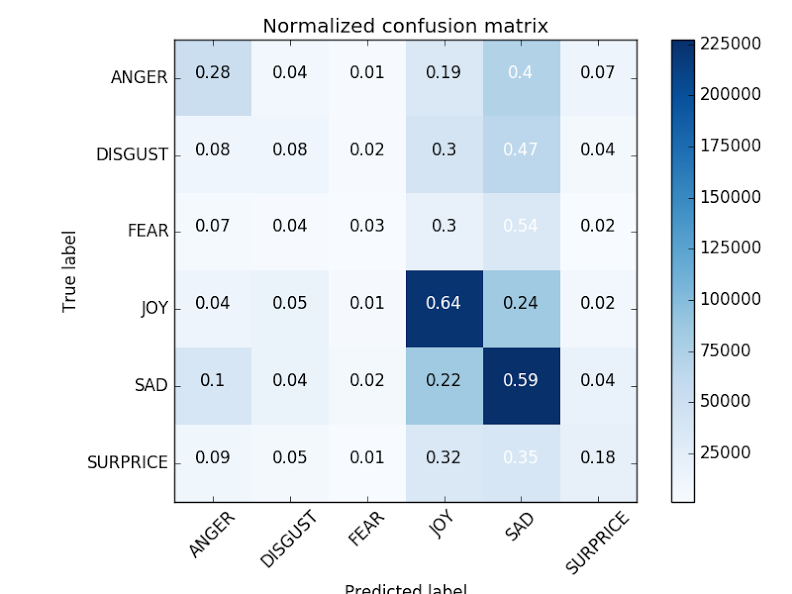
\includegraphics[width=1\linewidth]{tf-idf}
    \caption{The confusion matrix for TF-IDF+ SVM}
    \label{confusion1}
\end{figure}

\begin{figure}
\centering
\begin{subfigure}[b]{1\textwidth}
   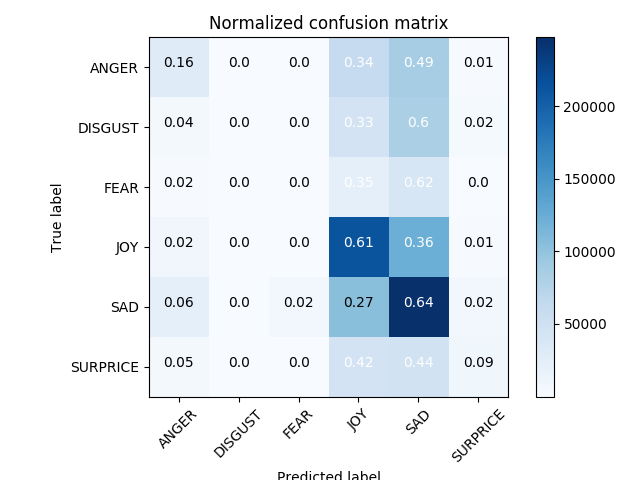
\includegraphics[width=.9\linewidth]{sc-ratio}
   \caption{}
   \label{confusion2} 
\end{subfigure}

\begin{subfigure}[b]{1\textwidth}
   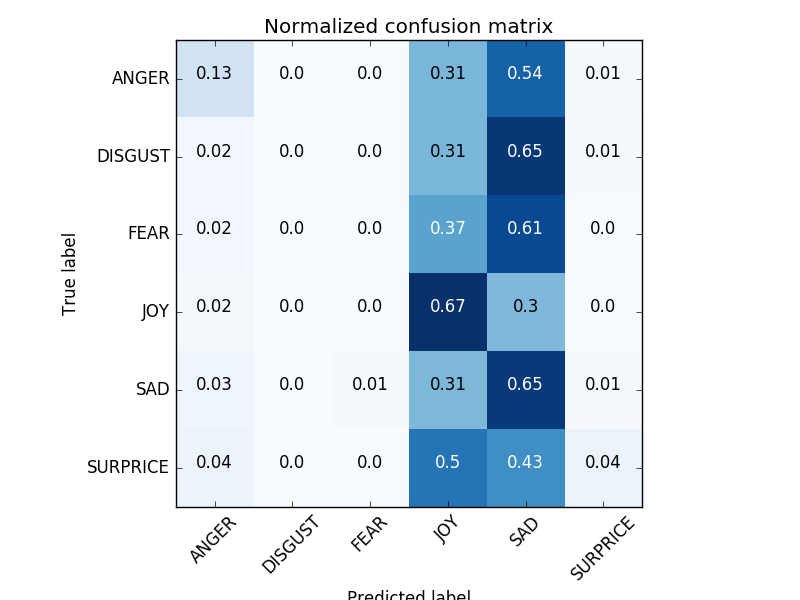
\includegraphics[width=.9\linewidth]{siamese-cbow-pretrained}
   \caption{}
   \label{confusion5}
\end{subfigure}
\caption[Confusion Matrix of Siamese-CBOW]{(a) The training set without pre-trained embedding,
(b) The training set with pre-trained embedding
}
\end{figure}


In the confusion matrix for fasttext in Figure \ref{confusion4}, it shows different tendancy for Pinyin dataset classification. 
The accuracy for SURPRICE is higher than SAD. It indicates that the SURPRICE may be modeled better than SAD, which contains more sample.

Figure \ref{confusion4} is quite similar with other confusion matrix, where most test data are classified as JOY and SAD.

\begin{figure}
\centering
\begin{subfigure}[b]{1\textwidth}
   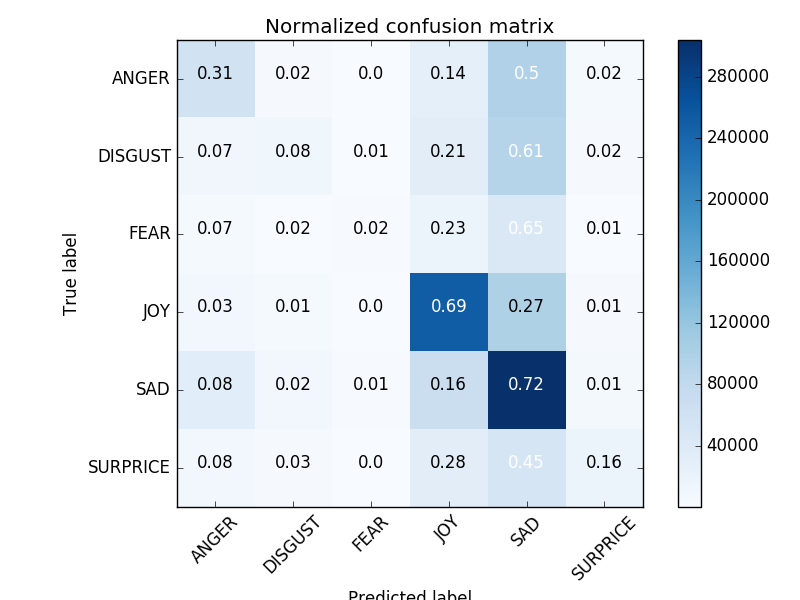
\includegraphics[width=.9\linewidth]{fasttext-All_seg_d300_w20_hs}
   \caption{}
   \label{confusion3} 
\end{subfigure}

\begin{subfigure}[b]{1\textwidth}
   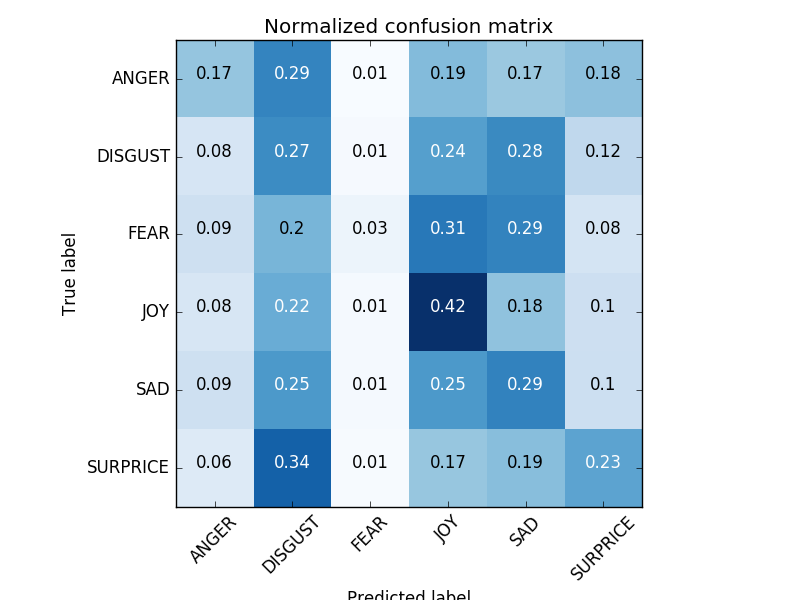
\includegraphics[width=.9\linewidth]{All_seg_d200_w15_softmax_pinyin}
   \caption{}
   \label{confusion4}
\end{subfigure}
\caption[Confusion Matrix of FastText]{(a) segmented dataset trained with dimension=300, window size=20, loss function hierarchical softmax,
(b) pinyin dataset with dimension=200, window size=15, and loss function = softmax
}
\end{figure}
